\begin{comment}
\begin{itemize}
  \item 全天球映像の表示方法自体を変更する手段として,宮藤ら\cite{10}のおかしら会議が挙げられる
  \item 球体ディスプレイそのものを顔として見立て,全天球映像の顔部分のみをマッピングする
  \item マッピングする際に,全天球パノラマ画像上下部分に見られる歪みを考慮し,修正する式を用いている
  \item (式を乗せて,どのように歪み補正が行われているかを説明)
  \item (アプリケーションが動いている様子も載せる)
\end{itemize}
\end{comment}

全天球映像の表示方法自体を変更する手段として,宮藤ら\cite{10}のおかしら会議が挙げられる.
これは球体ディスプレイそのものを顔として見立て,全天球映像の顔部分のみをマッピングするという手法である.

顔の切り抜きは,Dlibを用いて検出された顔バウンディングボックスによって行い,
拡大したのちに楕円形にトリミングする.その画像を背景が黒い長方形画像に張り付け,
正距方位図法への変換を行う.

この際,長方形にそのまま楕円顔画像を張り付けてしまうと,上下部分がが
相対的に小さく描画されてしまう.よって,その歪みを打ち消す処理を行っている.

\begin{figure}[tp]
  \centering
  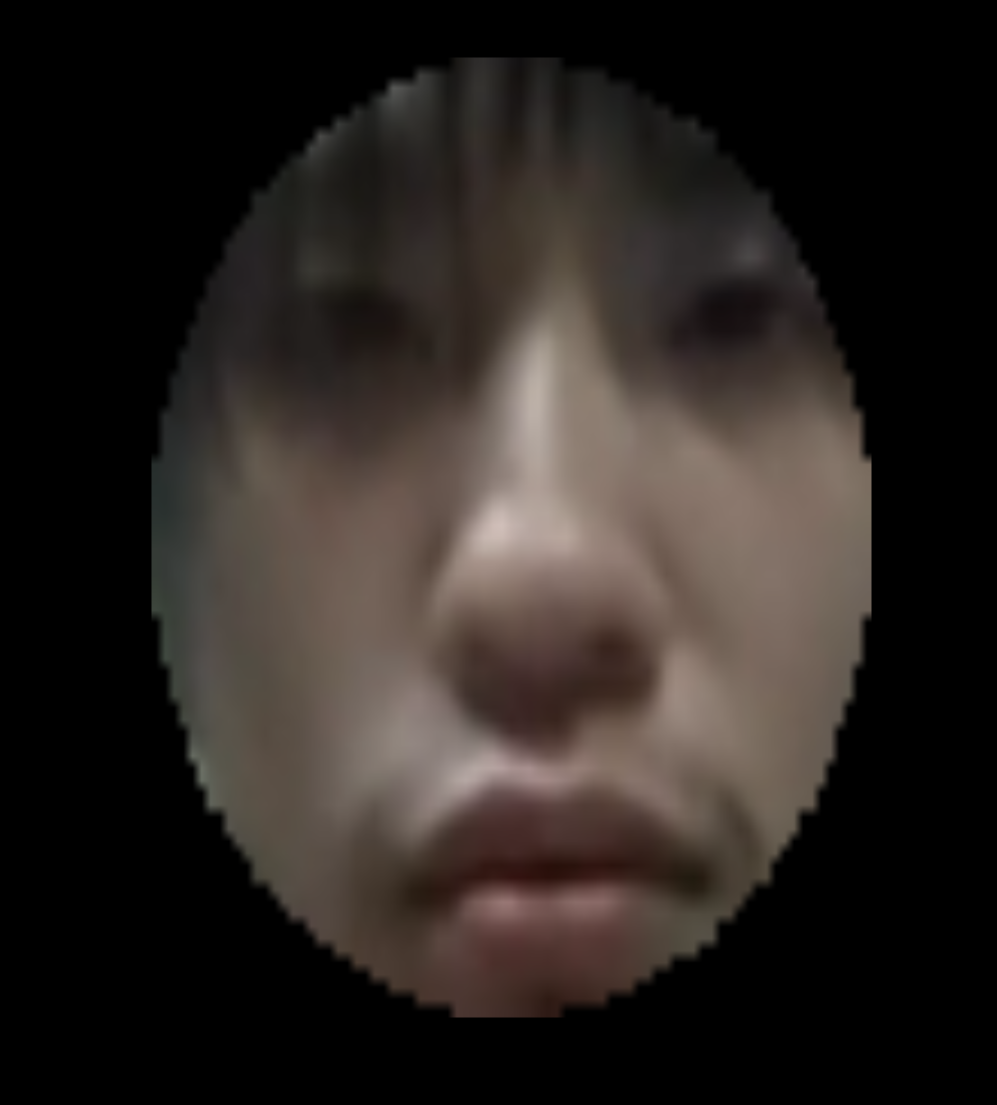
\includegraphics[scale=0.6]{fig/okashira1.png}
  \includegraphics[scale=0.1]{fig/okashira3.png}
  \caption{歪みの補正前}
\end{figure}

\begin{figure}[tp]
  \centering
  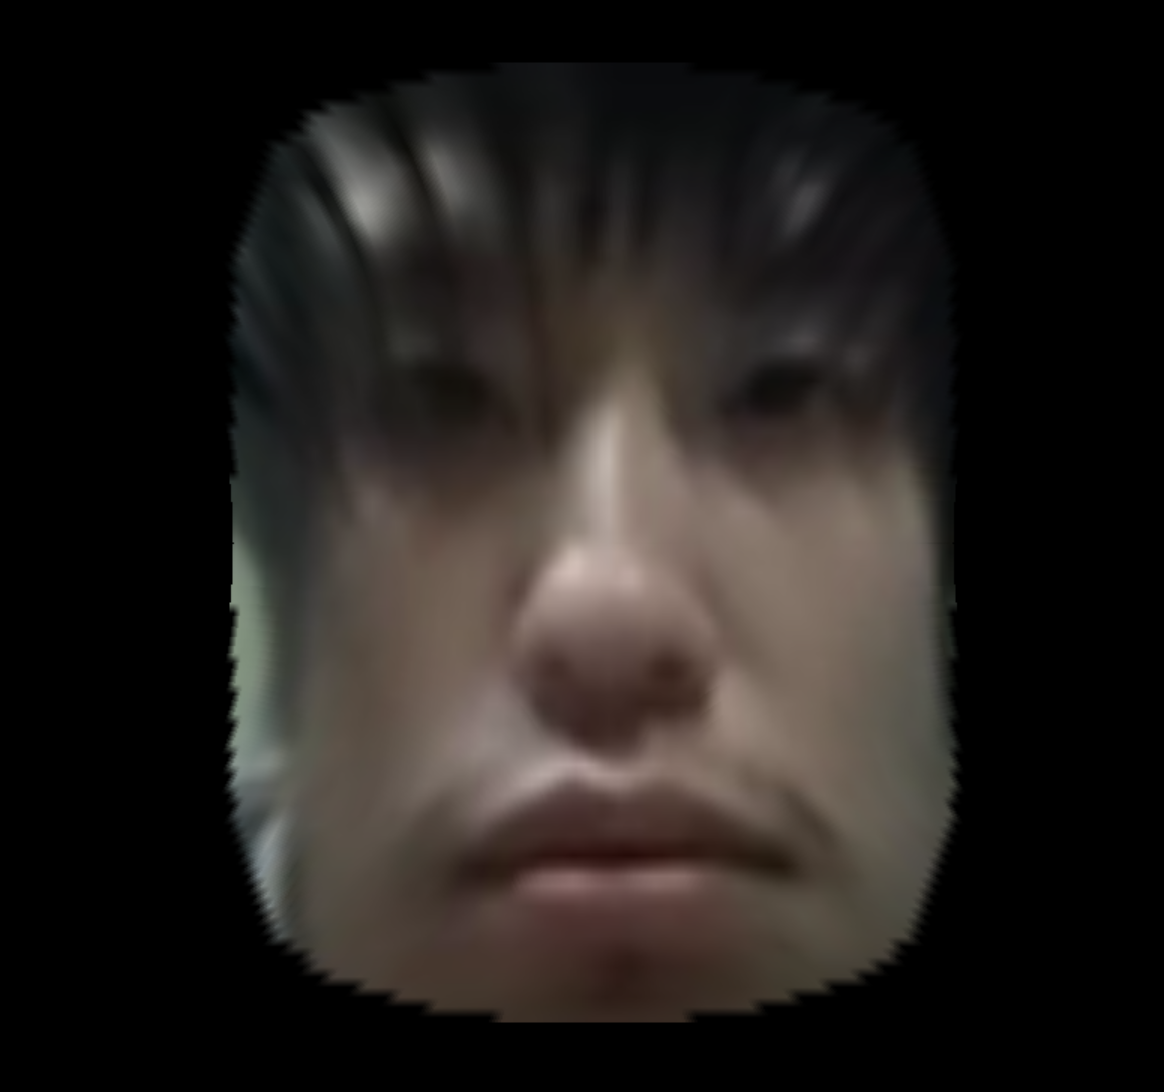
\includegraphics[scale=0.6]{fig/okashira2.png}
  \includegraphics[scale=0.1]{fig/okashira4.png}
  \caption{歪みの補正後}
\end{figure}

実験の考察でも述べた通り,立体的な資格情報は,
ビデオ会議での疑似的な対面経験を作り出すとみられる.
よって現実の顔に近い立体表現が可能なこの表示方法は
効果的であると考えられる.

問題点としては,全天球画像の顔の領域が小さいことが挙げられる.
小さい画像を拡大して大きな画像に張り付けるため,画質が著しく低下してしまう.

しかし,近年は4K画質に対応したカメラが多く存在し,全天球カメラにも
4K画質のものが存在する.GPUの性能向上と合わせ,高解像度のカメラ映像を遅延なく
送信することができれば,この問題は解決される.